\documentclass{report}
\usepackage{graphicx} % Required for inserting images
\usepackage[a4paper, margin = 2cm]{geometry}
\usepackage[none]{hyphenat}
\usepackage{parskip}
\usepackage{float}

\title{Astrodynamics for KSP}
\author{Andrew Kelly}
\date{October 2023}

\begin{document}

\maketitle
\chapter{Celestial Mechanics}

\section{Introductory relationships}

\subsection{Conic sections}
All trajectories are conic sections, which is the slice through two cones put tip to tip.

\begin{figure}[H]
    \centering
    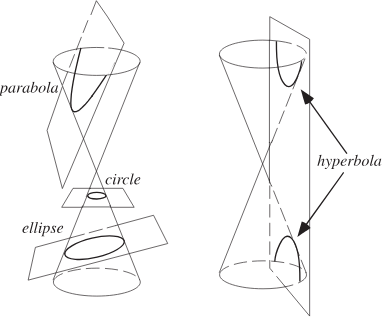
\includegraphics[width=0.5\linewidth]{Latex Images/ConicSection.png}
    \caption{Conic sections}
    \label{fig:conic}
\end{figure}

This means that despite the form of a trajectory, even a degenerate conic that intersects the nappe of the cone, has the same trajectory equation:
$$
r = \frac{p}{1+e \cos{(\nu)}}
$$
Here $r$ is the distance to the centre of the central body (not the surface!), $e$ is the eccentricity of the orbit, which characterises it, $p$ is the `semi-latus rectum' which is a length at 90$^\circ$ to the periapsis, and $\nu$ is the angle from the periapsis around the orbit.

\begin{figure}[H]
    \centering
    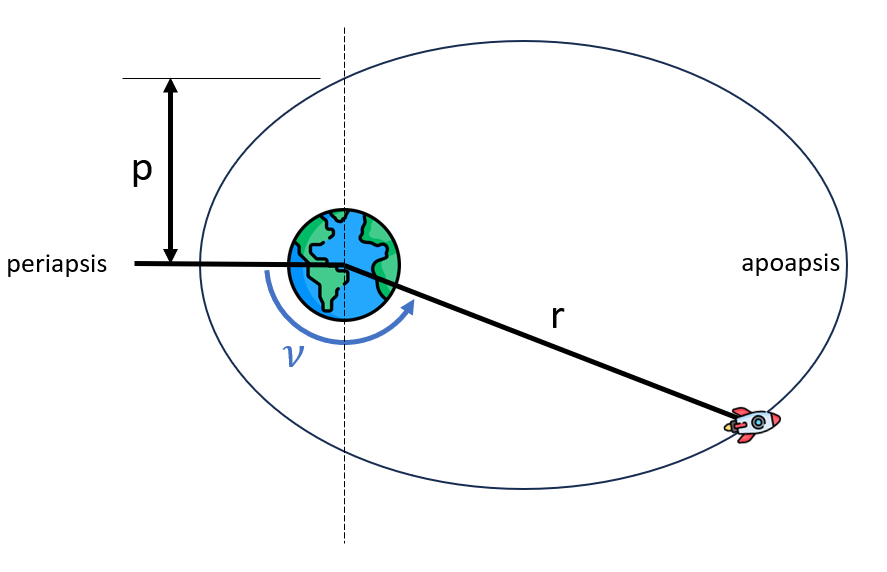
\includegraphics[width=0.7\linewidth]{Latex Images/Ellipse.png}
    \caption{Trajectry equation parts in an elliptical orbit}
    \label{fig:ellipse}
\end{figure}

The value of the semi-latus rectum is $p=h^2 /\mu$. Another relationship is $p = a(1-e^2 )$, or $e=\sqrt{1-p/a}$

Combined, the trajectory equation for all conic section orbits is:
$$
r = \frac{h^2}{\mu}\frac{1}{1+e\cos{(\nu)}}
$$

Note in figure \ref{fig:ellipse} that the planet is at one `focus' of the ellipse. This is true for all conic sections: There are always two focal points with the central body at one of them.

\subsection{Properties of conic-section orbits}

We first describe some equations and relationships that work for all orbits, and then we will later describe some specific geometries of the different conic sections.

\subsubsection{Conservation of mechanical energy}
The specific mechanical energy $\mathcal{E}$ of a satellite is the sum of its kinetic energy per unit mass, and its potential energy per unit mass. This is a constant in an orbit regardless of shape. 

$$
\mathcal{E} = \frac{v^2}{2}-\frac{\mu}{r}
$$

Where $v$ is the speed of the satellite at a specific point of an orbit, and $r$ is the distance from the centre of the central body with gravitational parameter $\mu$.

This is a useful term to calculate on an orbit as it also gives quick information on the shape. For an ellipse $\mathcal{E}<0$; for a parabolic trajectory $\mathcal{E}=0$; and for a hyperbolic trajectory $\mathcal{E}>0$.

Another relationship that is super useful is:

$$
\mathcal{E} = -\frac{\mu}{2a}
$$

\subsubsection{Conservation of angular momentum}
Angular momentum is also conserved in an orbit. In vector form:

$$
\vec{h} = \vec{r} \times \vec{h}
$$

Where $\vec{h}$ is a vector of the angular momentum, with $|h|$ being the value itself.

At periapsis (the closest point in the orbit to the central body) and apoapsis (the furthest point) we can use the values instead of the vectors, as here the position and velocity vectors are at right angles: $h = rv$ at these two points. Thus once you calculate $|h|$ you can work out the velocities at apo/peri quickly.

At a position different than the apo/periapsis, the velocity vector will not be tangent to the trajectory, and this difference is called the `flight path angle' $\phi$. Now, $h = rv \cos{(\phi)}$, with the sign of $\cos{(\phi)}$ being the same as the sign of $\vec{r} \cdot \vec{v}$.

\begin{figure}[H]
    \centering
    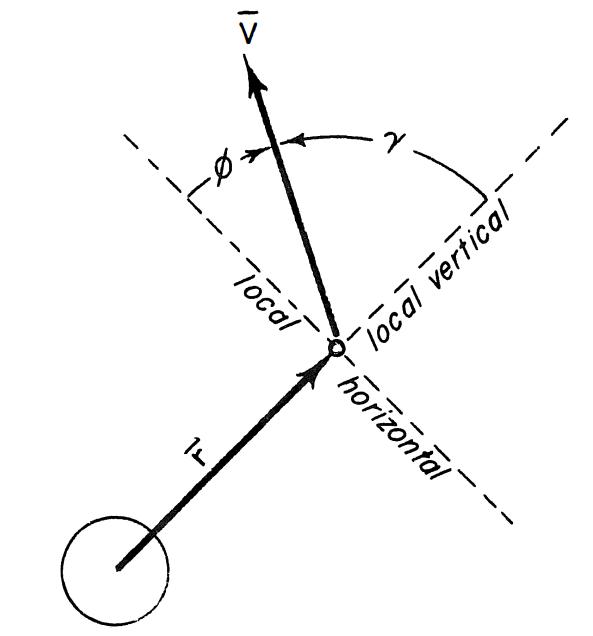
\includegraphics[width=0.4\linewidth]{Latex Images/flightpathangle.png}
    \caption{Flight path angle $\phi$}
    \label{fig:flightpath}
\end{figure}

There is a relationship combining specific mechanical energy and angular momentum:

$$
e = \sqrt{1+\frac{2\mathcal{E}h}{\mu ^2}}
$$

\subsubsection{Distance relations in conic orbits}

The distance at periapsis, $r_p$ and the distance at apoapsis, $r_a$, for any orbit can be determined from the semi-latus rectum or semi major axis, and the eccentricity:

$$
r_p = \frac{p}{1+e} = a(1-e), \quad r_p = \frac{p}{1-e} = a(1+e)
$$

\subsubsection{Velocity in conic orbits}

The velocity at any point on an orbit, regardless of shape, can be calculated from the "vis-viva" equation, also known as the `orbital-energy-invariance' law or Burgas' formula.

$$
v^2 = \mu \left({ 2 \over r} - {1 \over |a|}\right)
$$
Where $a$ is the semi-major axis of the orbit, the distance between the periapsis and apoapsis. The modulus is to handle the case of a hyperbola, which has a negative semi-major axis.

\subsubsection{Orbital period in conic orbits}

The orbital period, or the time taken to complete one orbit, is:

$$
T=2\pi\sqrt{a^3\over{\mu}}
$$

Actually calculating the time taken between two points is known as the `time of flight' problem and is fiendish. This will get its own section.

In terms of conic sections themselves, we will step through each one to describe the relevant geometry.

\subsection{Geometry specific to orbital shapes}

\subsubsection{Circular orbits}
For a circular orbit, the two focal points are at the centre. The semi-latus rectum is also equal to the radius, which is the same at all points of the trajectory. Each point on the circle is the periapsis (or apoapsis if you prefer), meaning we can always just use the momentum formula $h=rv$. The velocity at every point of a circular orbit is:

$$
v = \sqrt{\frac{\mu}{r}}
$$

\begin{figure}[H]
    \centering
    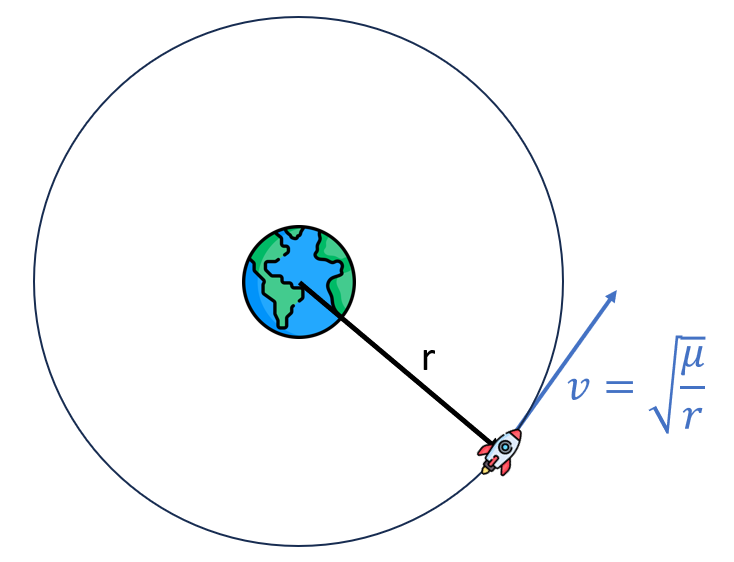
\includegraphics[width=0.5\linewidth]{Latex Images/circleorbit.png}
    \caption{Geometry of the circular orbit}
    \label{fig:circular}
\end{figure}

The escape velocity, or the new velocity required to make the trajectory parabolic from the starting radius $r$ is

$$
v = \sqrt{\frac{2\mu}{r}}
$$
In a circular orbit the eccentricity is zero, hence from the trajectory equation $r = p =h^2 /\mu$. The semi-major axis $a = 2r$ for a circle, and the specific mechanical energy $\mathcal{E}$ is negative.

\subsubsection{Elliptical orbits}
An ellipse is the last of the bound orbits, with the two focal points not being coincident, and the distance between them being finite.

For an elliptical orbit, the eccentricity is $0<e<1$. 

A key property of ellipses is that the sum of the distances from any point to both foci is constant, and equal to twice the semi major axis. Considering the periapsis and apoapsis distances this means $2a = r_p + r_a$. As a consequence:

$$
a = \frac{p}{1-e^2}
$$

and

$$
e = \frac{r_a - r_p}{r_a + r_p}
$$

The specific mechanical energy $\mathcal{E}<0$, as for all bound orbits. 

\begin{figure}[H]
    \centering
    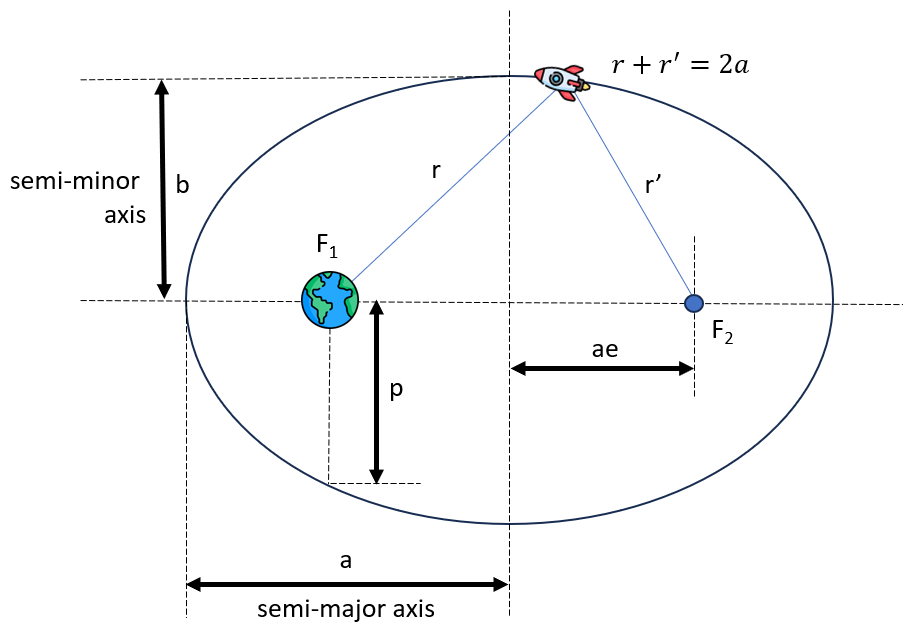
\includegraphics[width=0.8\linewidth]{Latex Images/EllipticalOrbit.png}
    \caption{Geometry of the elliptical orbit}
    \label{fig:EllipticalOrbit}
\end{figure}

\subsubsection{Parabolic orbits}

A parabolic orbit is defined as having one focus at infinity. As such $a = \infty$ and $e=1$, and $\mathcal{E} = 0$. Because of the extreme precision of the parameters exact parabolic trajectories are almost never found, but they are useful to know the details of as the bifurcation point between bound and unbound orbits.

As $e=1$, the periapsis distance is just $r_p = p/2$. $r_a = \infty$.

The speed anywhere on the parabolic orbit it:

$$
v = \sqrt{\frac{2\mu}{r}}
$$

\begin{figure}[H]
    \centering
    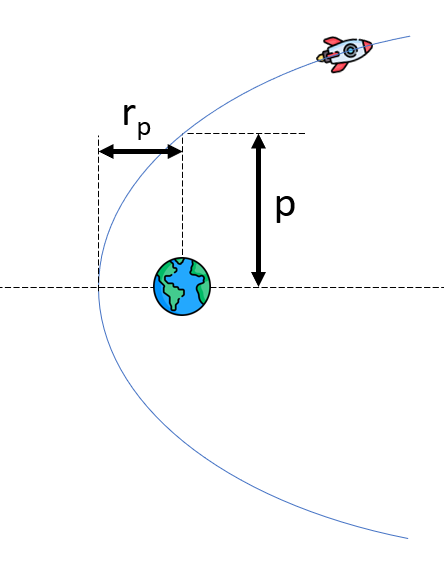
\includegraphics[width=0.3\linewidth]{Latex Images/ParabolicOrbit.png}
    \caption{Geometry of the parabolic orbit}
    \label{fig:parabolicorbit}
\end{figure}

\subsubsection{Hyperbolic orbit}
Hyperbolic orbits are the classical unbound orbit. A hyperbola as a mathematical object has two `lobes', but in an actual orbit the path travels on only one of them. There are two foci, but only one is relevant.

For a hyperbola, $e>1$, $a<0$ and $\mathcal{E}>1$. 

The denominator of the trajectory equation goes to zero when $\cos{(\nu)} = -1/e$. This angle which can be called $\nu_{\infty}$ is the `true anomaly of the asymptote'. Another relationship for this is $\sin \nu _{\infty }={\frac {1}{e}}{\sqrt {e^{2}-1}}$

The angle between the two asymptotes is called is `turning angle' $\delta$, and a relation is $\sin{(\delta/2)}= 1/e$

There is a property called the `hyperbolic excess speed'. If a satellite has exactly enough speed to escape the gravity of a body, it will be a parabolic orbit, and at infinity the satellite will have velocity zero. For a hyperbolic orbit, the velocity it will have at the hypothetical infinity is the `hyperbolic excess speed'. This can be determined from the specific mechanical energy, $\mathcal{E} = v_{\infty}/2$

\begin{figure}[H]
    \centering
    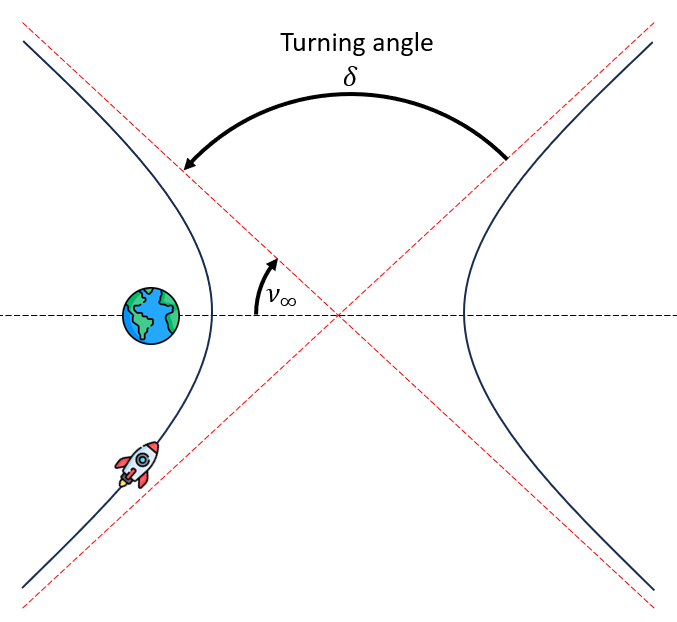
\includegraphics[width=0.5\linewidth]{Latex Images/HyperbolicOrbit.png}
    \caption{Geometry of a hyperbolic orbit}
    \label{fig:hyperbolic}
\end{figure}

\subsection{Sphere of influence}
Naturally, satellites don't get to infinity away. We can talk about a `sphere of influence', where when an object reaches a certain distance from the body the effect of gravity becomes so low that we can consider the object to be free from the influence of the body. This is especially the case when there are multiple bodies: as you approach a new body that one exerts a larger gravitational influence, and eventually you can consider only this one body, and ignore the previous one.

In KSP these are defined for each body. This is useful as it makes an n-body problem a 1-body problem. Once you know when you are a certain distance from a body and have crossed the sphere of influence, you can simply switch all of your equations over to referring to that body. To do this by hand requires knowledge of radius and velocity vectors and full orbital parameters.

\begin{figure}[H]
    \centering
    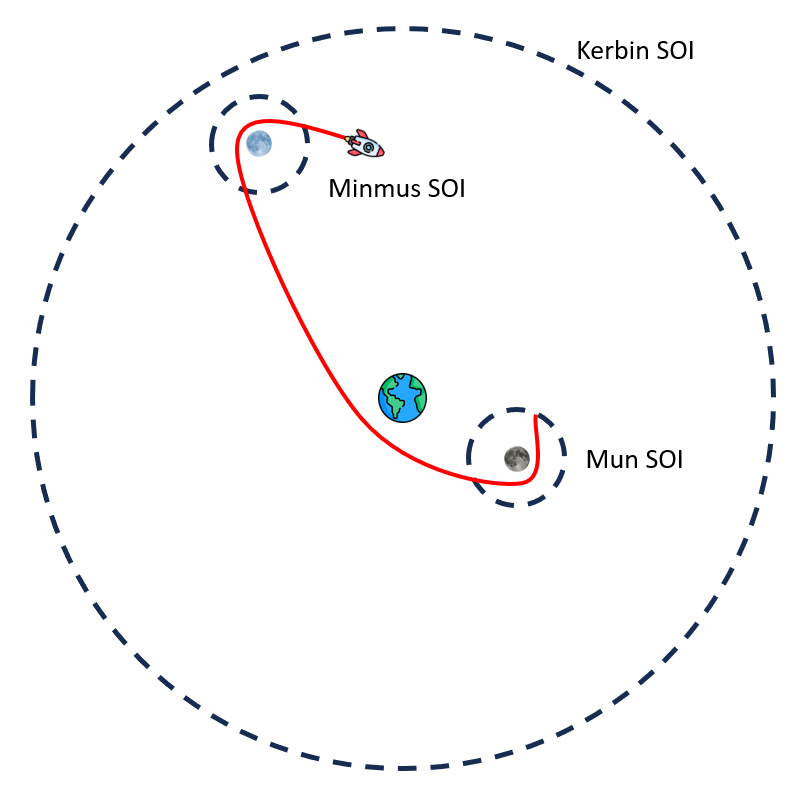
\includegraphics[width=0.5\linewidth]{Latex Images/SphereOfInfluence.png}
    \caption{A trajectory crossing multiple spheres of influence (not to scale)}
    \label{fig:SOI}
\end{figure}

\section{Time of flight problems}

Orbital period is easy. Time of flight (TOF) is hard because the speed changes around an orbit.

\subsection{Mean and eccentric anomaly}
We start by defining the 



\section{Canonical units}
Before moving on to vectors, we can simplify the work by using `canonical units'.

A `reference orbit' is an orbit just grazing the surface of the planet. If we define this to be our distance unit (DU), with TU being the time unit describing the orbital period of this reference orbit. When doing this, we simplify as $\mu = 1$. 

Sometimes this is useful... but it's a throwback to the old days. Nowadays computational power is cheap.

\chapter{Coordinate systems and orbital parameters}
For any body, we can describe its position and velocity using vectors. All vectors, however, require a reference frame.

\section{Coordinate systems}
\subsection{Heliocentric/ecliptic coordinate system}
Kerbol can be origin of your system, and then describe X and Y coordinates with regards a reference position, which is the line between Kerbol and Kerbin when the epoch starts. The Y axis is defined using the right-hand rule. 

\begin{figure}[H]
    \centering
    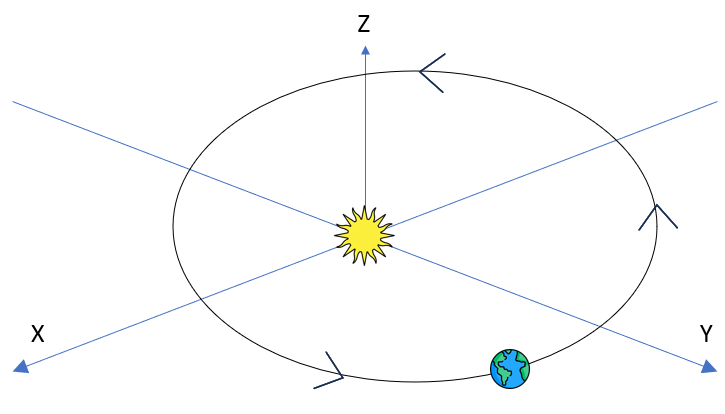
\includegraphics[width=0.5\linewidth]{Latex Images/Heliocentric.png}
    \caption{Heliocentric/Ecliptic coordinate system}
    \label{fig:enter-label}
\end{figure}

This is sometimes called the `ecliptic' system of coordinates, as the orbital plane is called the `ecliptic' and sometimes notated as $(X_{\epsilon},Y_{\epsilon},Z_{\epsilon})$ An orbit can be inclined out of the ecliptic, but this will be covered later.

\subsection{Geocentric coordinate system}
If the central body is a planet, it is a geocentric coordinate system. We spend most of our time in this system, only using the ecliptic system when considering where the main planets of the system will at some point in the future.

Along the X direction we can define the unit $\hat{I}$ vector, similarly with $\hat{J}$ and $\hat{K}$.

\begin{figure}[H]
    \centering
    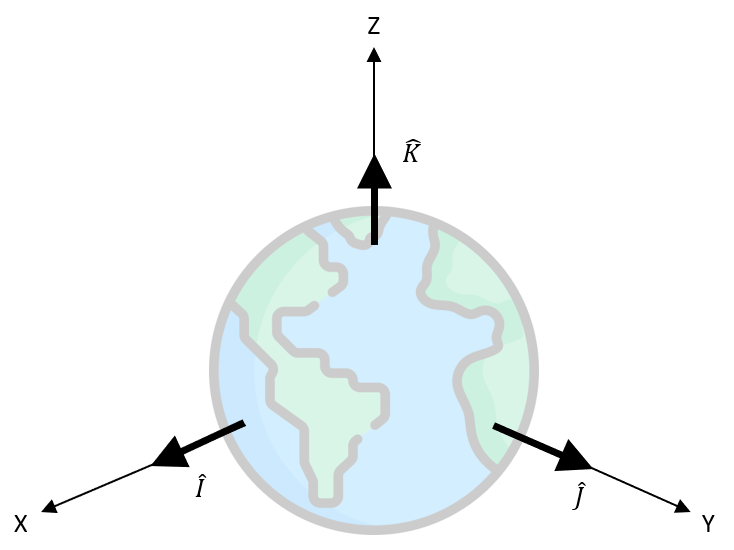
\includegraphics[width=0.5\linewidth]{Latex Images/Geocentric.png}
    \caption{Geocentric coordinate system}
    \label{fig:geocentric}
\end{figure}



\subsubsection{Eccentricity vector}
The eccentricity vector for any orbit is:

$$
\vec{e} = \frac{\vec{v} \times \vec{h}}{\mu}-\frac{\vec{r}}{r}
$$
Another formulation is easier to calculate, not needing $\vec{h}$ or the cross product:
$$
\mu \vec{e} = \bigg(v^2-\frac{\mu}{r}\bigg)\vec{r}-(\vec{r}\cdot\vec{v})\vec{v}
$$

\end{document}

